\documentclass[windows,csize4, answers]{BHCexam}
%\documentclass[windows,csize4,answers]{BHCexam}

\usepackage{multicol} % 分栏
\usepackage{polynom} % 多项式除法
\pagestyle{fancy}
\fancyfoot[C]{\kaishu \small 第 \thepage 页 共 \pageref{lastpage} 页}
%\fancyhead[L]{\includegraphics[width=2cm]{qrcode.png}}
\title{声音}
%\subtitle{数学文科试卷}
%\notice{满分150分, 120分钟完成, \\	允许使用计算器,答案一律写在答题纸上.}
%\author{Gavin Chen}
%\date{\today}
\usepackage{enumerate} % 编号
\usepackage{cases}
\usepackage{subfigure}
\usepackage{graphicx}

\begin{document}

\maketitle

\begin{groups}
    \group{光的直线传播}{}
    \begin{itemize}
        \item 光在同种均匀介质中沿直线传播。(为什么?费马原理,最小作用量原理,变分法。)
        \item 直线传播的例子:影子,月食,日食,小孔成像。
        \item 光源的概念:能发出一定波长范围的电磁波(包括可见光以及紫外线、红外线和X射线等不可见光)的物体。
        \item 冷光源和热光源:一般来说,冷光源发光不会对周围温度产生明显变化。通常利用化学能,生物能来转化为光能。而热光源通常发光同时也会发热。
        \item 自然光源,人造光源。
    \end{itemize} 

    光源发光照到不透明物体后,在物体背光面形成的光所达不到的区域即为影子。
    影区是发自光源并于被照物体相切的光线围成的。图\ref{fig:fig_3_1}(a)中,点光源形成的影。如果把点光源改成面光源,如图\ref{fig:fig_3_1}(b)所示。
    注意这时候情况会有所不同,后面的影区氛围本影(完全照不到)和半影(部分照到)。
    想一想,假如图\ref{fig:fig_3_1}(b)中光源为圆形,的半影区有个人往光源看,他看到的光源是什么形状?
    \begin{figure}[htb]
        \centering
        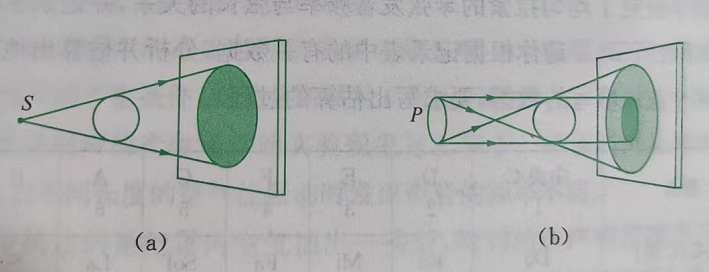
\includegraphics [scale=0.75,trim=0 0 0 0]{./image/fig_3_1.PNG}
        \caption{点光源与面光源的影}
        \label{fig:fig_3_1}
    \end{figure}

    图\ref{fig:fig_3_2}所示为日食情况。a为本影区,看到日全食;c、d为半影区,看到日偏食;而b为伪本影区,看到日环食。
    \begin{figure}[htb]
        \centering
        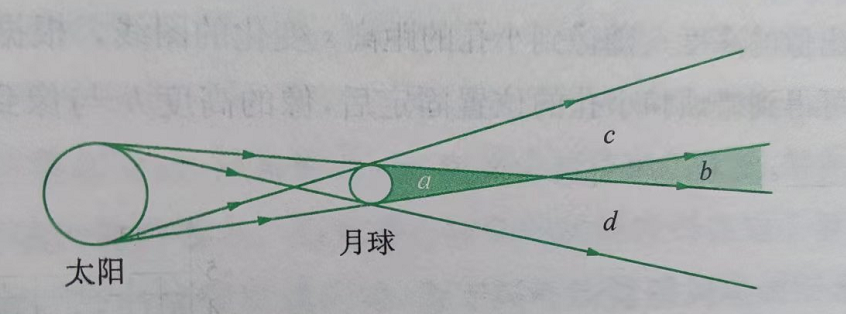
\includegraphics [scale=0.75,trim=0 0 0 0]{./image/fig_3_2.PNG}
        \caption{日食}
        \label{fig:fig_3_2}
    \end{figure}
    图\ref{fig:fig_3_3}所示为月食情况。想一想,为什么没有月环食?
    \begin{figure}[htb]
        \centering
        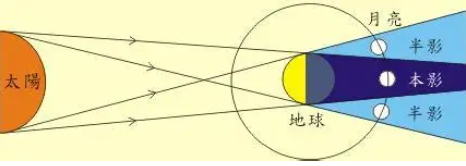
\includegraphics [scale=0.75,trim=0 0 0 0]{./image/fig_3_3.PNG}
        \caption{月食}
        \label{fig:fig_3_3}
    \end{figure}






    \group{例题}{}

    \begin{questions}[]
        \question[5]无
        \begin{solution}{0.5cm}
            \methodonly a
        \end{solution}
 

    \end{questions}

    \group{作业}{}
    \begin{questions}[]

        \question[5] 假
        \begin{solution}{0.5cm}
            \methodonly 
        \end{solution}



    \end{questions}
















\end{groups}




\label{lastpage}
\end{document}